\documentclass[11pt,a4paper]{article}
\usepackage[margin=2.2cm]{geometry}
\usepackage[T1]{fontenc}
\usepackage{charter}
\usepackage{microtype}
\usepackage{graphicx}
\usepackage{booktabs}
\usepackage{array}
\usepackage{tabularx}
\usepackage{float}
\usepackage{caption}
\usepackage{enumitem}
\usepackage{amsmath}
\usepackage[table]{xcolor}
\usepackage{listings}
\usepackage[most]{tcolorbox}
\usepackage{fancyhdr}
\usepackage[colorlinks=true,linkcolor=accent,urlcolor=accent]{hyperref}

\definecolor{accent}{HTML}{3C3489}
\definecolor{codebg}{HTML}{F6F6F3}
\definecolor{kw}{HTML}{185FA5}
\definecolor{cm}{HTML}{6B6A64}
\definecolor{okgreen}{HTML}{0F6E56}
\definecolor{badred}{HTML}{A32D2D}

\setlength{\parindent}{0pt}
\setlength{\parskip}{6pt}
\setlist{itemsep=2pt,topsep=4pt}
\captionsetup{font=small,labelfont=bf}
\renewcommand{\arraystretch}{1.18}

\pagestyle{fancy}\fancyhf{}
\rhead{\small\color{cm}\reporttag}
\cfoot{\small\thepage}
\renewcommand{\headrulewidth}{0.3pt}

\lstdefinelanguage{SV}{
  morekeywords={module,endmodule,input,output,inout,logic,wire,reg,always_ff,always_comb,assign,
    begin,end,if,else,case,endcase,default,typedef,enum,localparam,posedge,negedge,or,task,endtask,
    function,endfunction,automatic,initial,repeat,while,for,integer,string,signed,void},
  sensitive=true, morecomment=[l]{//}, morecomment=[s]{/*}{*/}, morestring=[b]"}
\lstdefinelanguage{ICCTcl}{
  morekeywords={set_app_var,create_mw_lib,open_mw_lib,import_designs,read_sdc,set_tlu_plus_files,
    save_mw_cel,create_floorplan,derive_pg_connection,create_rectangular_ring,create_power_strap,
    create_fp_placement,place_opt,clock_opt,report_placement_utilization,report_qor,report_timing,
    insert_stdcell_filler,route_opt,verify_zrt_route,extract_rc,write_parasitics,write_verilog,
    close_mw_cel,gui_start,set_dont_use,get_lib_cells},
  sensitive=true, morecomment=[l]{\#}}
\lstset{basicstyle=\ttfamily\footnotesize, backgroundcolor=\color{codebg}, frame=single,
  rulecolor=\color{codebg}, keywordstyle=\color{kw}\bfseries, commentstyle=\color{cm}\itshape,
  columns=fullflexible, keepspaces=true, breaklines=true, showstringspaces=false,
  xleftmargin=4pt, xrightmargin=4pt, aboveskip=6pt, belowskip=6pt}

\newtcolorbox{task}{colback=accent!5,colframe=accent,boxrule=0.6pt,arc=2pt,
  left=8pt,right=8pt,top=4pt,bottom=4pt,fonttitle=\bfseries,title=The assignment}
\newtcolorbox{keypoint}[1]{colback=okgreen!6,colframe=okgreen,boxrule=0.6pt,arc=2pt,
  left=8pt,right=8pt,top=4pt,bottom=4pt,fonttitle=\bfseries,title={#1}}
\newtcolorbox{lesson}[1]{colback=orange!7,colframe=orange!70!black,boxrule=0.6pt,arc=2pt,
  left=8pt,right=8pt,top=4pt,bottom=4pt,fonttitle=\bfseries,title={#1}}

\newcommand{\fig}[3]{\begin{figure}[H]\centering\includegraphics[width=#2\linewidth]{figures/#1}\caption{#3}\end{figure}}
\newcommand{\met}{\textcolor{okgreen}{\textbf{MET}}}
\newcommand{\viol}{\textcolor{badred}{\textbf{VIOLATED}}}
% numbers still to be copied from my own .rpt files (shows in red until filled in)
\newcommand{\fillin}[1]{\textcolor{badred}{\textbf{[#1]}}}

\newcommand{\header}[3]{%
  \begin{center}
  {\small\color{cm} CPE 527 VLSI Design \quad|\quad Lab 3 \quad|\quad University of Alabama in Huntsville}\\[8pt]
  {\LARGE\bfseries\color{accent} #1}\\[4pt]
  {\large #2}\\[8pt]
  {\small Bibek Shrestha \quad|\quad October 2026 \quad|\quad #3}
  \end{center}\vspace{2pt}\hrule\vspace{6pt}}
\newcommand{\reporttag}{Lab 3 / Assignment 3: MSP430 multiplier place and route}

\begin{document}
\header{Place and Route of the MSP430 Hardware Multiplier}{Taking the Lab 2 netlist through IC Compiler}{Synopsys IC Compiler, SAED 90\,nm}

\begin{task}
Run the IC Compiler flow from the tutorial on a design from the previous lab: floorplan, power plan,
placement, clock tree synthesis and routing. Generate and analyze the reports after CTS and after routing.
\end{task}

\section*{At a glance}
\begin{table}[H]\centering\small
\begin{tabular}{lccc}
\toprule
 & \textbf{Lab 2 (DC)} & \textbf{After CTS} & \textbf{After routing} \\
\midrule
Library corner & typ & max & max \\
Wires & none & estimated & routed + extracted \\
Clock & 7 ns & 7 ns & 7 ns \\
Critical path & 6.91 ns & \fillin{ns} & \fillin{ns} \\
Setup slack & 0.00 ns & \fillin{ns} & \fillin{ns} \\
Violating paths & 0 & \fillin{} & \fillin{} \\
Hold violations & & \fillin{} & \fillin{} \\
Cells & 881 & \fillin{} & \fillin{} \\
Cell area & 12677.53 & \fillin{} & \fillin{} \\
Utilization & & \fillin{\%} & \fillin{\%} \\
Open nets / DRCs & & & \fillin{} / \fillin{} \\
\bottomrule
\end{tabular}
\caption{Lab 2 synthesis next to the two ICC checkpoints.}
\end{table}

\section{The design}
The same \texttt{mult430} from Lab 2: a memory-mapped 16$\times$16 multiplier (MPY, MPYS, MAC, MACS) on a
shared tri-state data bus. It has two submodules, the control FSM \texttt{u\_ctrl} and the datapath \texttt{u\_dp}.
The 32-bit adder inside the datapath was the critical path in Lab 2.

\fig{arch.png}{0.78}{Architecture from Lab 2.}

Ports: \texttt{clk}, \texttt{reset\_n}, \texttt{addr[15:0]}, \texttt{data\_bus[15:0]} (inout),
\texttt{write\_enable}, \texttt{read\_enable}, \texttt{busy}. That is 52 signal pins, compared with 7 for the gray counter.

\section{Script changes}
The script is the tutorial flow with new names, plus one addition.

\begin{table}[H]\centering\small
\begin{tabular}{ll}
\toprule
Tutorial & This design \\
\midrule
\texttt{gray4bcntLIB} & \texttt{MULT\_LIB} \\
\texttt{gray\_counter.ddc}, top \texttt{gray\_counter} & \texttt{assignment3.ddc}, top \texttt{mult430} \\
\texttt{gray\_counter.sdc} (5 ns) & \texttt{assignment3.sdc} (7 ns) \\
checkpoints \texttt{gray4bcnt\_*} & \texttt{MULT\_init}, \texttt{MULT\_cts\_opt}, \texttt{MULT\_route} \\
 & \texttt{set\_dont\_use} on \texttt{BSLEX1/2/4} \\
\bottomrule
\end{tabular}
\caption{Differences from the tutorial script.}
\end{table}

In Lab 2 the BSLEX tri-state cells gave wrong gate-level results, so Design Compiler was told not to use them
and picked \texttt{TNBUFFX} instead. \texttt{place\_opt} and \texttt{route\_opt} can resize or swap cells while fixing
timing, and they do not know about the Lab 2 ban, so the same \texttt{set\_dont\_use} lines are repeated in ICC.

\section{Flow, stage by stage}
\fig{icc_stages.png}{1.0}{(1) After import the cells are stacked outside the core. (2) The floorplan sizes the core;
the cells wait in rows beside it. (3) VSS/VDD rings and straps. (4) Rough placement fills the core.
(5) After \texttt{clock\_opt} the first routed nets (green) are the clock tree. (6) Filler cells close the row gaps.}

Compared with the gray counter, the core is much larger: the same 0.6 utilization now has to hold 881 cells
instead of 15, so the die grows while the 30\,\textmu m ring margin stays the same.

\section{Routed layout}
\begin{figure}[H]\centering
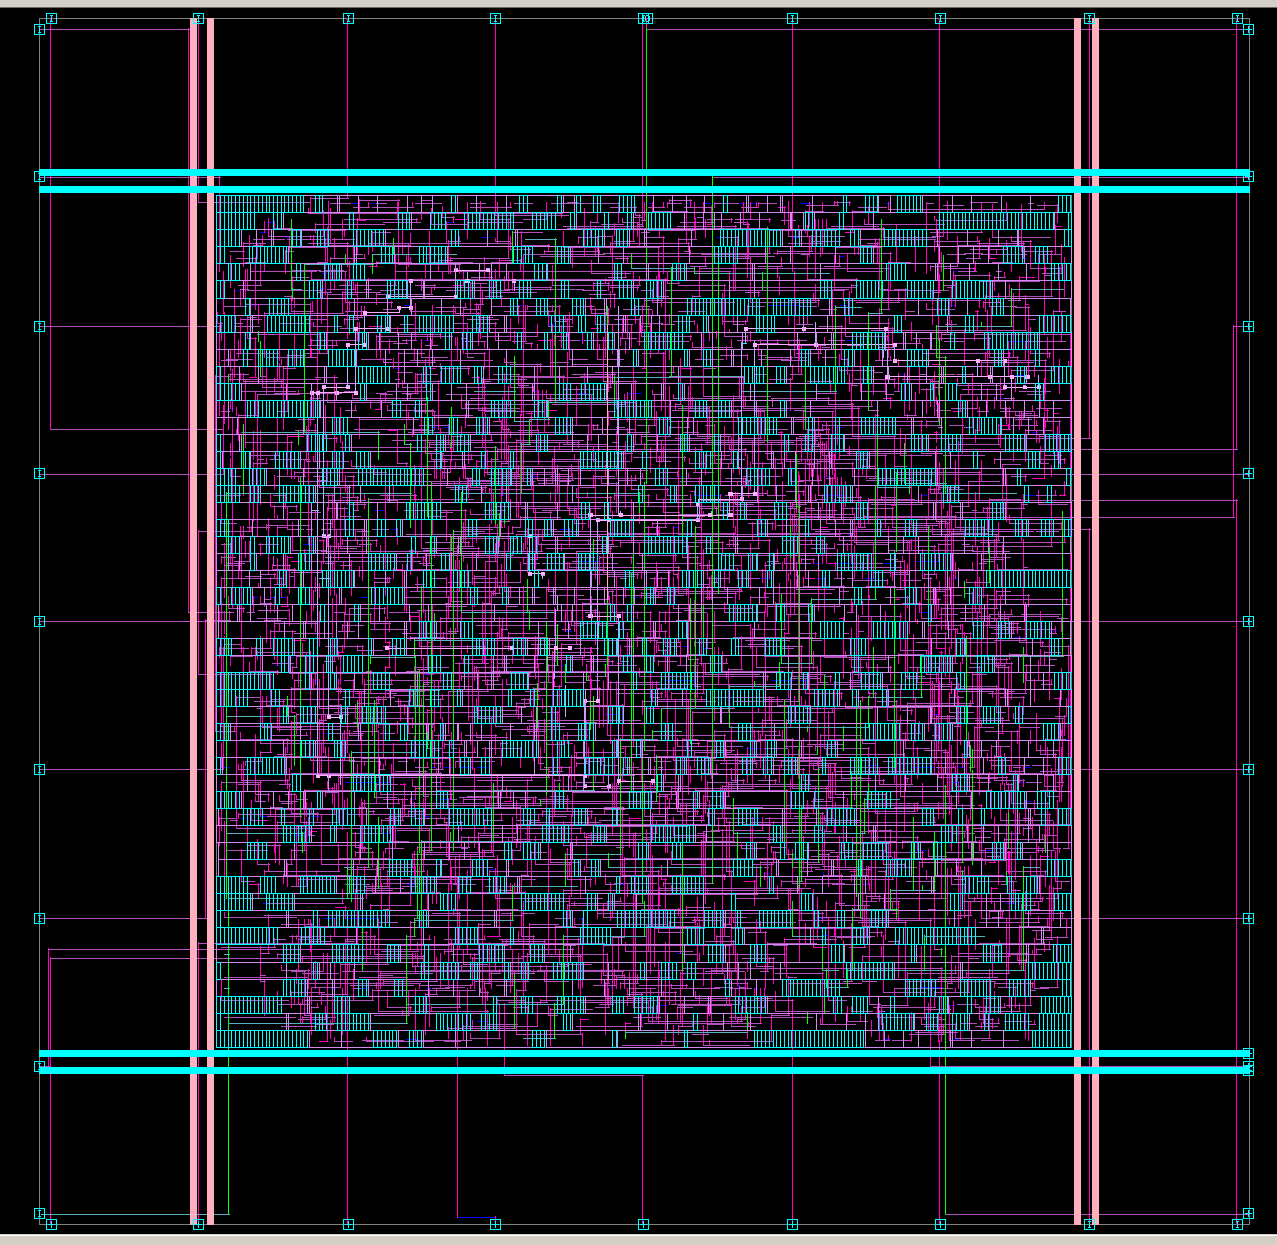
\includegraphics[width=0.48\linewidth]{figures/icc_routed.png}\hfill
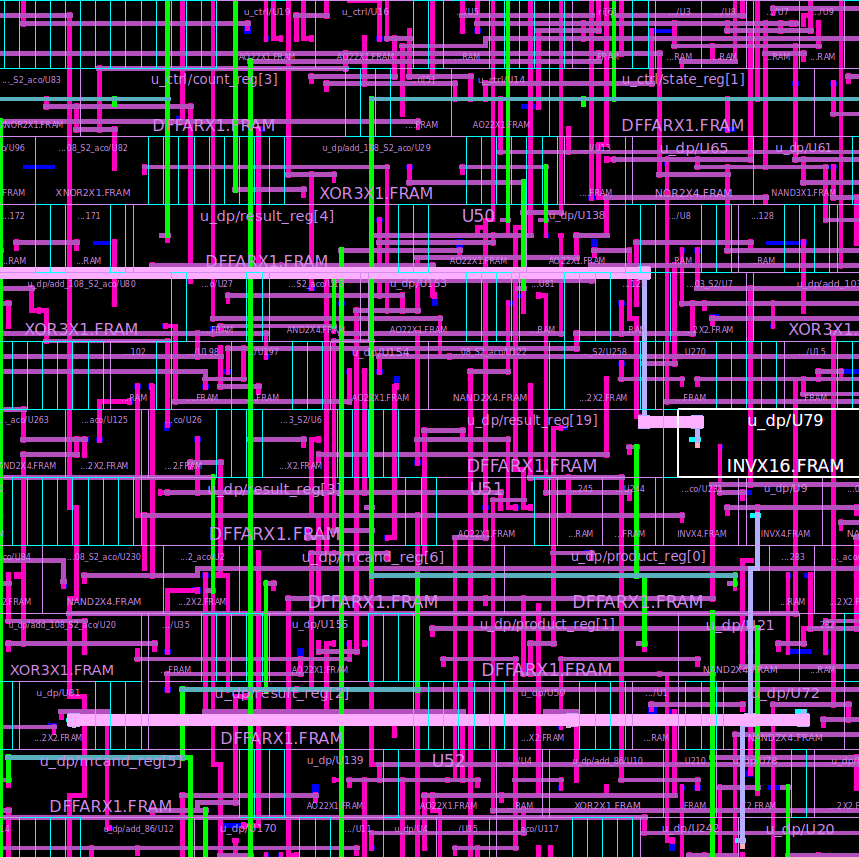
\includegraphics[width=0.48\linewidth]{figures/icc_routed_zoom.png}
\caption{Left: the full routed block. Right: a zoom. The instance names keep the RTL hierarchy:
\texttt{u\_ctrl/state\_reg}, \texttt{u\_ctrl/count\_reg}, \texttt{u\_dp/product\_reg}, \texttt{u\_dp/result\_reg},
\texttt{u\_dp/mcand\_reg}, and \texttt{u\_dp/add\_108\_52} for the adder Design Compiler built.}
\end{figure}

\section{Reports}
\begin{table}[H]\centering\small
\begin{tabular}{lll}
\toprule
Report & What I checked & Result \\
\midrule
\texttt{MULT\_route\_qor.rpt} & slack, violating paths & \fillin{} \\
\texttt{MULT\_route.setup.rpt} & worst setup path & \fillin{start $\rightarrow$ end, slack} \\
\texttt{MULT\_route.hold.rpt} & worst hold path & \fillin{} \\
\texttt{MULT\_route\_util.rpt} & standard cell utilization & \fillin{} \\
\texttt{verify\_zrt\_route} & open nets, DRCs & \fillin{} \\
\bottomrule
\end{tabular}
\caption{Post-route reports.}
\end{table}

\begin{lesson}{Why the timing is different from Lab 2}
Lab 2 had exactly 0.00\,ns of slack at 7\,ns, but that was with the \emph{typical} library and no wires.
ICC checks the \emph{max} (slow) corner and, after routing, adds real wire R and C.
Both make the 32-bit carry chain slower, so the post-route slack is \fillin{ns}.
\end{lesson}

\section{Inside the cells}
\begin{figure}[H]\centering
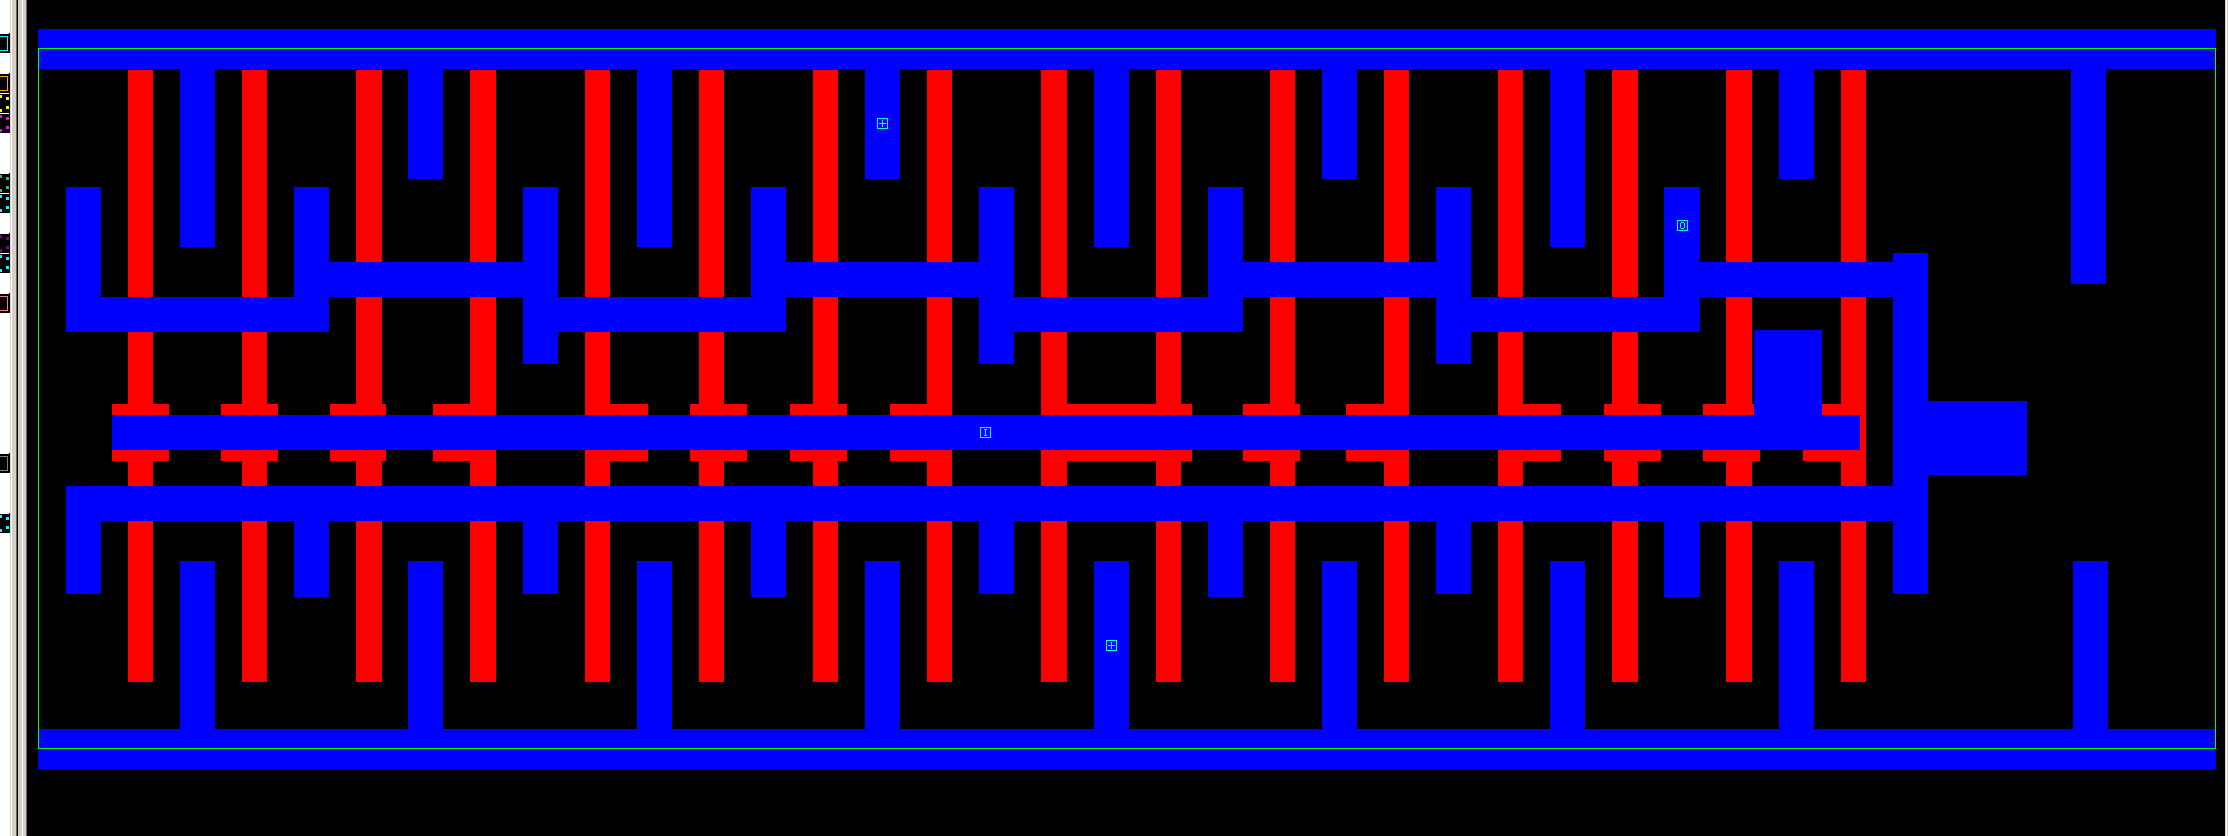
\includegraphics[width=0.49\linewidth]{figures/icc_invx16_fram.png}\hfill
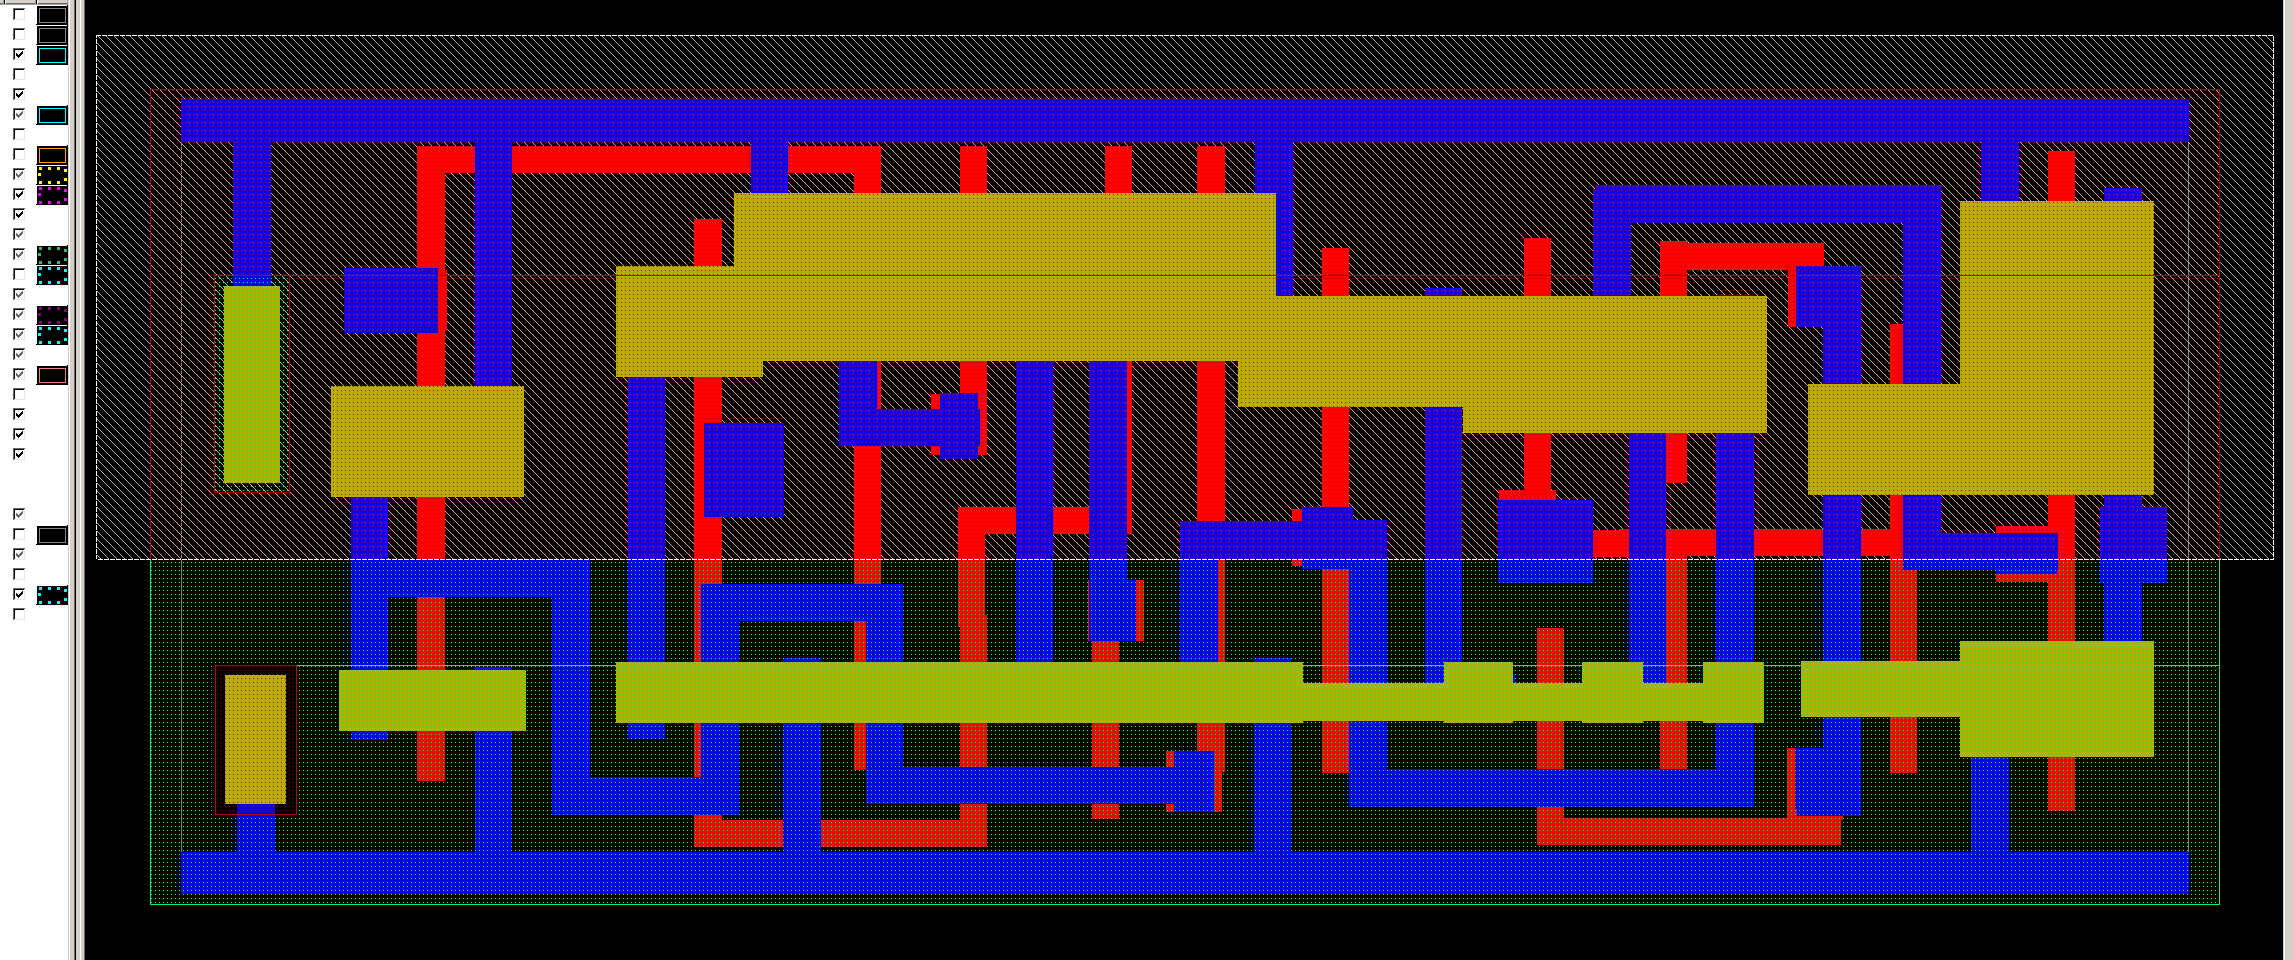
\includegraphics[width=0.49\linewidth]{figures/icc_xor3x1_cel.png}
\caption{Left: \texttt{INVX16} (instance \texttt{u\_dp/U79}), FRAM view. It is 16 inverters in parallel: the
repeated red poly fingers share one input and one output, which gives the high drive strength.
Right: \texttt{XOR3X1}, CEL view, with the N-well (hatched) on top for the PMOS and the NMOS below.}
\end{figure}

\section{What I learned}
\begin{itemize}
\item Physical design is where the real timing shows up. A path with 0.00\,ns slack after synthesis has no room
      left for the slow corner or for wire delay.
\item The hierarchy (\texttt{u\_ctrl}, \texttt{u\_dp}) survives into the layout, which makes it easy to find a
      register in the GUI.
\item Constraints set in Design Compiler, like \texttt{set\_dont\_use}, are not carried into ICC automatically.
\item A larger design takes much longer to draw and route; ``REDRAW INTERRUPTED'' in the GUI is just the
      display giving way to the running command.
\end{itemize}

\appendix
\section{Source files}
\subsection*{RTL: \texttt{src/assignment3.sv}}
\lstinputlisting[language=SV]{src/assignment3.sv}
\subsection*{Testbench: \texttt{src/assignment3\_tb.sv}}
\lstinputlisting[language=SV]{src/assignment3_tb.sv}
\subsection*{ICC script: \texttt{src/icc\_mult.tcl}}
\lstinputlisting[language=ICCTcl]{src/icc_mult.tcl}
\end{document}
